\section{\label{sec:newdesign}Subsequent New Design}

% hex arrangement
\begin{figure}[ht]
    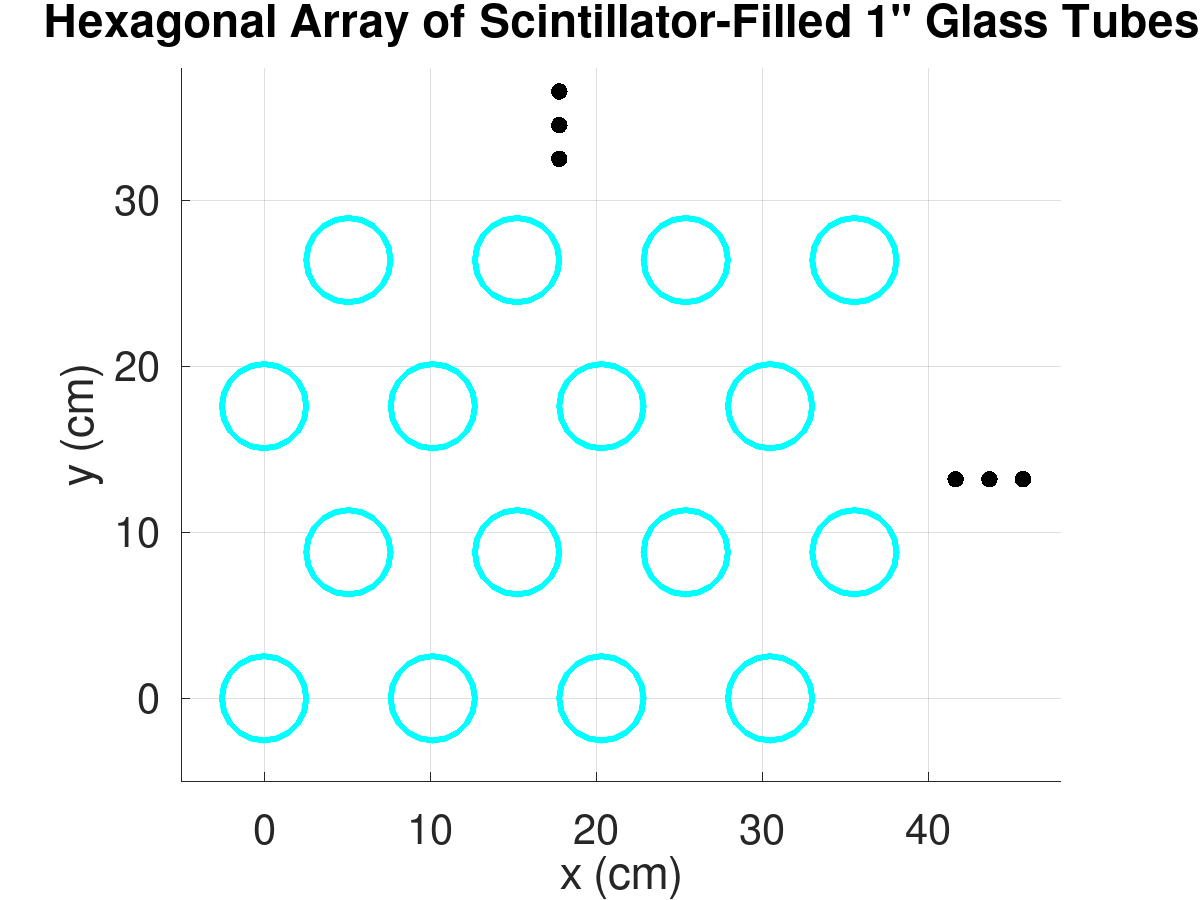
\includegraphics[width=0.8\linewidth]{figures/forest_top.png}
    \caption{Array Pattern for Proposed Hybrid Design}
    \label{fig:forest_top}
\end{figure}

% tube array
\begin{figure}[ht]
    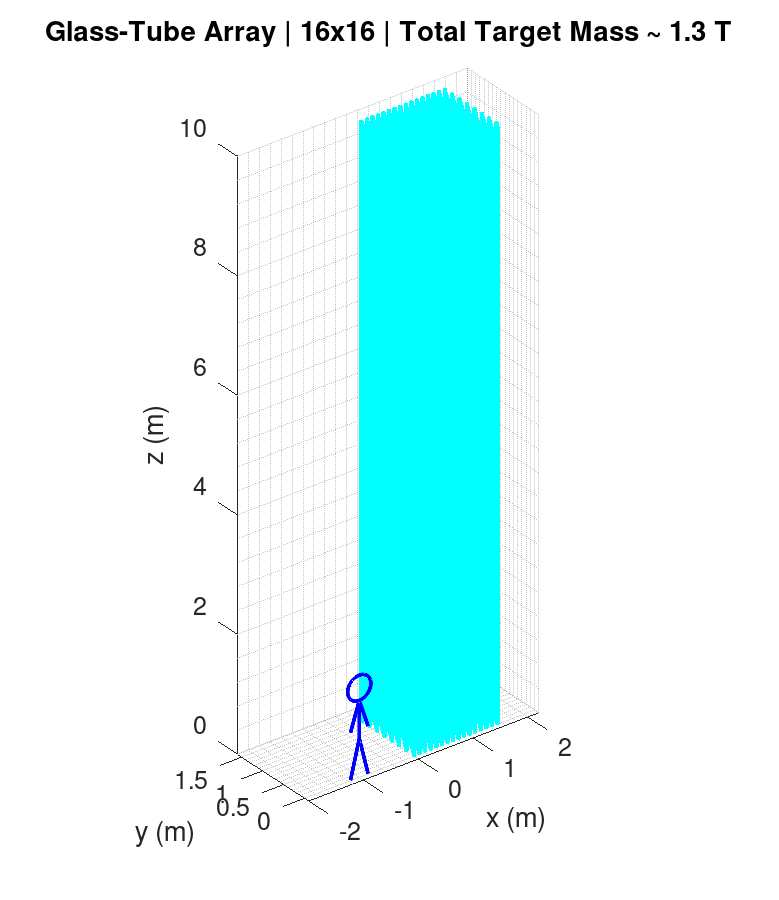
\includegraphics[width=0.8\linewidth]{figures/forest_h.png}
    \caption{Scaled Rendering of Proposed Hybrid Design}
    \label{fig:forest_full}
\end{figure}

In our efforts to emulate the superb angular resolution of the impractical SANTA design, we considered how to allow the neutron to fly freely once the proton is transformed, and how to subsequently record the capture location.
%Two facts work for us here.
%First, if we can limit the thickness of the proton-rich interaction medium (the scintillator), then the neutron may escape before ``forgetting'' its production direction.
%Second, while traversing the free-flight region, the neutron will take some time to reach the capture location, and we can readily measure this time if it is even a few~cm, due to the non-relativistic velocity $(\sim\nicefrac{c}{10^3}$) of the neutron; the kinetic energy in this case is just $\nicefrac{1}{2}mv^2$. 
%If we determine both the time and location of capture relative to the positron production, we will approach the SANTA-style directional determination.
To this end, our first design constraint was to limit the thickness of the proton-rich scattering medium (\textit{i.e.}, the scintillator), to increase the average distance the neutrons travel before their first scatter.
This separates the neutron-scattering and -capture region from the \ibd\ vertex and is the primary mechanism behind \santa's outstanding directional performance.
Our other primary design consideration was to approach the comparatively large target mass and strong background resilience (relative to \santa) demonstrated or predicted in the other detector designs.

To balance these opposing requirements, we decided on an array of vertical glass tubes containing liquid scintillator.
The reason for employing glass tubes (preferably quartz) is the lack of free protons; this allows the neutrons to penetrate glass with little scattering.
% This would not be the case with plastic tubes which would be simpler and less expensive.
Plastic tubes, which would be more cost-effective and simpler to use, unfortunately do not share this advantage.
% TODO (?): include comparative cross-section plot   jgl: naah

We therefore contrived a ``forest'' of vertical scintillator-filled tubes with light detectors at each end. (PMT of better SiPMs with cooling)
% The strength of glass tubes is such that even 10m long tubes provide no pressure (around one atmosphere) challenge to commercially available pipes.
Commercially-available glass is strong enough to easily contain the scintillator, even at a tube length of 10~m, where the differential pressure at the bottom is $(\sim 1~\mathrm{atm})$.
The same is true of the end windows on the bottom, adjacent to the lower light detectors.

We want an open array allowing a few~cm of flight path for the neutron to travel before encountering another cylinder. 
We have postulated either alternating tubes, with and without dopant, or possibly employing dopant in all tubes and depending upon the short distance to the surface to allow frequent neutron escape after production.

A subsection of the scintillator array demonstrating the geometrical arrangement is shown in Fig.~\ref{fig:forest_top}.
A simple scaled rendering of the full array is shown in Fig.~\ref{fig:forest_full}.

The key to determining the viability of this configuration will depend on efficiency and angular resolution.
We have run several sets of initial simulations to investigate this design's performance.
In order to get the best comparison of directional capability with the other simulated designs, we have used the same thouroughly-tested \rat\ material we used for the other hybrid detectors: PVT plastic scintillator doped at $1.5\%\mathrm{wt}\ \nucl{6}{Li}$ \dash see Tab.~\ref{tab:ncomp_results}.
We are currently testing options for the final design.
(Note: The phase of the scintillator material has little-to-no impact on its directional performace; only the number densities of scattering targets and capture nuclei are relevant).
See Fig.~\ref{fig:ref_results} in \S~\ref{sec:deltaphi} below for our initial results for tubes of $\sim$2.54-cm diameter spaced 1~diameter apart in a hexagonal lattice.
The angular resolution appears quite attractive to further study.

We also note that it may be possible to record the time and location of the neutron's first scatter after exiting the tube in which it was produced.
(In a typical event, this happens when it enters the tube in which it will eventually capture).
This would allow us to determine additional information about the neutron's kinematics, which are nonrelativistic in these interactions ($KE_n\sim10^{0}~\mathrm{kEV}$).
It would require timing resolution and especially scintillator light output that push the bounds of what is currently available but is nevertheless at least plausible.

In sum, we think this novel geometry may lead to a practical directional \ibd\ detector, but significant study both in simulation and in the laboratory is still needed.
